%%
% Please see https://bitbucket.org/rivanvx/beamer/wiki/Home for obtaining beamer.
%%
%\documentclass[11pt,aspectratio=169]{beamer}
%\documentclass[11pt,aspectratio=169,xcolor={dvipsnames}]{beamer}

\documentclass[11pt,aspectratio=169,xcolor={dvipsnames},hyperref={pdftex,pdfpagemode=UseNone,hidelinks,pdfdisplaydoctitle=true},usepdftitle=false]{beamer}
\usepackage{presentation}


\title{Lecture 18: Empirics of the Q Theory}
\author{Juan Herre\~{n}o\\UCSD}
\date{2026}

% Enter presentation title to populate PDF metadata:
\newcommand{\Cov}{\text{Cov}_\lambda}
\newcommand{\El}{\mathbb{E}_\lambda}
\newcommand{\mm}{\text{{\fontfamily{qzc}\selectfont m}}}
\usepackage{cancel}
\usepackage{booktabs}
\begin{document}

\begin{frame}
  \titlepage
\end{frame}

\begin{frame}{Lessons from last lecture}
\begin{itemize}
\item We saw last lecture that in our simple model
$$\frac{I_t}{K_t} = \frac{q_t - 1}{\varphi}$$
\vspace{-0.5cm}
\pause
\item And in more general specifications
$$\frac{I_t}{K_t} = h(q_t)$$
\vspace{-0.5cm}
\pause
\item Where $q_t$ is the marginal value of an additional unit of capital (marginal q)
\pause
\item i.e. $\partial V_t/ \partial K_{t+1}$, where $V$ is the value of the firm
\pause
\item If the following assumptions hold:
\begin{itemize}
\item The production function is CRS
\item The adjustment cost function is CRS
\item Markets are competitive
\end{itemize}
\item Then Average $Q$ is equal to marginal $q$, where
$$Q_t = \frac{V^e_t}{K_t}$$ 
\end{itemize}
\end{frame}

\begin{frame}{Empirical Implications of the Q-Theory}
$$\frac{I_t}{K_t} = h(q_t)$$
\vspace{-0.5cm}
\pause
\begin{itemize}
\item Q-Theory implies that $Q$ is a \textit{sufficient statistic} for firm investment
\pause
\item In english: the expected NPV (discounting with $r$) of marginal projects is the only determinant of investment
\pause
\item In english: The market value relative to book value of the firm encodes the NPV of the marginal projects
\pause
\item No other variable should explain investment on top of $Q$
\pause
\item i.e. cash flows, liquidity, size of the firm should be irrelevant after controlling for $Q$
\end{itemize}
\end{frame}


\begin{frame}{What is the alternative to the Q-Theory?}
\begin{itemize}
\item Breaking several of the assumptions, breaks the result:
\pause
\begin{itemize}
\item $q$ is a sufficient statistic
\item  $Q_t = q_t$
\end{itemize}
\pause
\item A prominent alternative is that capital markets are not perfect
\pause
\begin{itemize}
\item The internal cost of funds is higher than the external cost of funds
\pause
\item This may happen due to asymmetric information
\pause
\item You are experts on this
\end{itemize}
\pause
\item Another alternative is that adjustment costs are not CRS
\begin{itemize}
\item We will also talk about that extensively
\end{itemize}
\pause
\item In these cases, investment may be determined by current cash flows
\begin{itemize}
\item Firms that generate large cash flows have more internal funds
\item Lower cost of funds as a result
\item And may invest more
\end{itemize}
\end{itemize}
\end{frame}


\begin{frame}
Today:
\begin{itemize}
\item Are departures from the $Q$ Theory economically meaningful?
\pause
\item How strongly investment reacts to changes in the cost of capital?
\end{itemize}
\end{frame}

\begin{frame}{Why are these questions important}
\begin{itemize}
\item What is the effect of tax policy on investment and GDP growth?
\pause
\item How large is the ``investment-channel'' of monetary policy?
\pause
\item Do our models capture investment movements correctly?
\pause
\item Should we explore other models?
\pause
\end{itemize}
\end{frame}



\begin{frame}{What is the ideal regression?}
\begin{itemize}
\item We take our model
$$\frac{I_{it}}{K_{it}} =  \frac{q_{it} - 1}{\varphi}$$
\pause
\vspace{-0.5cm}
\item And run the regression:
$$\frac{I_{it}}{K_{it}} = \beta_0 + \beta_1 Q_{it}  + \epsilon_{it}$$
\vspace{-0.5cm}
\pause
\item so $\beta_0 =  - \frac{1}{\varphi}$, and $\beta_1 = \frac{1}{\varphi}$
\item Summers (1981) estimated this equation using OLS, finding $\hat{\beta_1} = 0.031$, $se_{\hat{\beta}_1} = 0.005$
\pause
\item Implying $\hat{\varphi} = 32.25$
\end{itemize}
\end{frame}


\begin{frame}{Research Design}
\begin{itemize}
\item Regression equation
$$\frac{I_{it}}{K_{it}} = \beta_0 + \beta_1 Q_{it}  + \epsilon_{it}$$
\item Simulateneity problem
\begin{itemize}
\item Higher $q$ calls for higher investment rates
\item Higher investment rates increase future capital stocks
\item Reducing future MPKs
\item Reducing $q$
\end{itemize}
\item Not clear what direction of causality this regression is exploiting
\begin{itemize}
\item Ideally we need exogenous variation in $q$
\end{itemize}
\end{itemize}	
\end{frame}



\begin{frame}{Smell Test}
\begin{itemize}
\item The first issue with the empirics of the $Q$ theory is that it requires values of $\varphi$ that are difficult to believe
\pause
\item Economics: Investment does not react to changes in $Q$
\pause
\item The model rationalizes this by making it very costly to change the capital stock
\pause
\item What do models that attempt to fit investment rates data say about $\varphi$?
\pause
\begin{itemize}
\item Cooper and Haltiwanger (2006) use $\varphi = 0.049$ using annual data
\item Winberry (2021) uses $\varphi = 2.49$ using quarterly data
\item Compare to the $\hat{\varphi} = 32$ in Summers (1981) using annual data
\pause
\item Caution: this parameter is not trivial to compare across different time dimensions
\end{itemize}
\end{itemize}
\end{frame}

\begin{frame}{What is $\epsilon_{it}$}
\begin{itemize}
\item The large implied adjustment costs are not the only problem
\pause
$$\frac{I_{it}}{K_{it}} = \beta_0 + \beta_1 Q_{it}  + \epsilon_{it}$$
\vspace{-0.5cm}
\pause
\item Where did $\epsilon_{it}$ came from?
\pause
\item The $Q$ theory is supposed to hold exactly
\pause
\item To think about the identification challenges of $\beta$ we need to think about the sources of variation of $\epsilon_{it}$
\pause
\item Key question: Is $\epsilon_{it}$ orthogonal to $Q_{it}$?
\end{itemize}
\end{frame}

\begin{frame}{Two interpretations}
\begin{itemize}
\pause
\item $\epsilon_{it}$ is measurement error of investment rates
\pause
\begin{itemize}
\item But perhaps the denominator of $Q$ is mismeasured as well?
\pause
\item Book value does not capture replacement cost
\pause
\item Measurement error would cause attenuation bias on $\beta_1$
\pause
\item Explaining its low value
\end{itemize}
\item The model is wrong, and other factors beyond $Q$ matter
\pause
\begin{itemize}
\item Would this cause bias on $\beta_1$?
\pause
\item It would if uncontrolled factors are correlated with $Q$
\pause
\begin{itemize}
\item Imagine a factor that determines investment \textit{beyond} $Q$
\pause
\item But helps determining $Q$ as well: example (interest rates, current productivity, current cash flow)
\end{itemize}
\pause
\item The sign of the bias is difficult to predict. Depends on the source of omitted variation
\end{itemize}
\end{itemize}
\end{frame}

\begin{frame}{Testing the $Q$ theory}
\begin{itemize}
\item Only $Q$ should matter
\pause
\item Insight: Compare firms with differential access to financial markets
\pause
\item Why?
\pause
\item One prominent economic alternative to the $Q$ theory is that financial access matters to determine investment
\pause
\item Evidence against the null of $Q$ as a sufficient statistic
\pause
\item Is this logic sound enough?
\end{itemize}
\end{frame}

\begin{frame}{Investment excess sensitivity to cash flows}
\begin{itemize}
\item Imagine we are interested in knowing whether cash flows affect investment \textit{on top of} $Q$
\pause
\item Simple approach
$$\frac{I_{it}}{K_{it}} = \alpha + \beta_1 Q_{it} + \beta_2 \frac{CF_{it}}{K_{it}} + \epsilon_{it}$$
\pause
\item Issue
\pause
\item Imagine $Q$ is mismeasured ...
\pause
\item Cash flows today may be correlated with future profitability or future investment opportunities
\pause
\item then cash flows and $Q$ are correlated
\pause
\item $\beta_2$ will pick-up variation driven by $Q$
\pause
\item Even when the $Q$ theory holds
\end{itemize}
\end{frame}

\begin{frame}{Moral}
Measurement error is really no joke
\end{frame}


\begin{frame}{Fazzari Hubbard Petersen (1988)}
\begin{itemize}
\item Idea: Use a difference-in-differences strategy to circumvent the cash flow - future profitability correlation problem
\pause
\item Split firms in groups that capture extent of financial constraints
\pause
\begin{itemize}
\item Firms that pay high versus low dividends
\end{itemize}
\pause
\item Compare sensitivity to cash-flows across groups
\pause
\item Identifying assumption
\begin{itemize}
\item $Q$ is not differentially mismeasured across groups
\pause
\item Capital adjustment costs are not sorted in the dividend-payment dimension
\end{itemize}
\end{itemize}
\end{frame}

\begin{frame}{Fazzari Hubbard Petersen (1988)}
\begin{itemize}
\item The empirical specification is more general
$$\frac{I_{it}}{K_{it}} = \alpha_t + \gamma_i + \beta_1 Q_{it} + \beta_2 \frac{CF_{it}}{K_{it}} + \epsilon_{it}$$
\item Run regression for each dividend bin separately
\pause
\item Could have done an interaction term as well
\pause
\item Sample: 1970-1984
\item Firm fixed effects: Captures firm-level differences in investment rates across firms
\item Time fixed-effects: Captures whatever aggregate shock that affects all the firms in the same group
\pause
\item This regression by group has a triple-difference flavor. $\beta_2$ is already a dif-dif.
\end{itemize}
\end{frame}

\begin{frame}{Fazzari Hubbard Petersen (1988)}
\begin{figure}
\centering
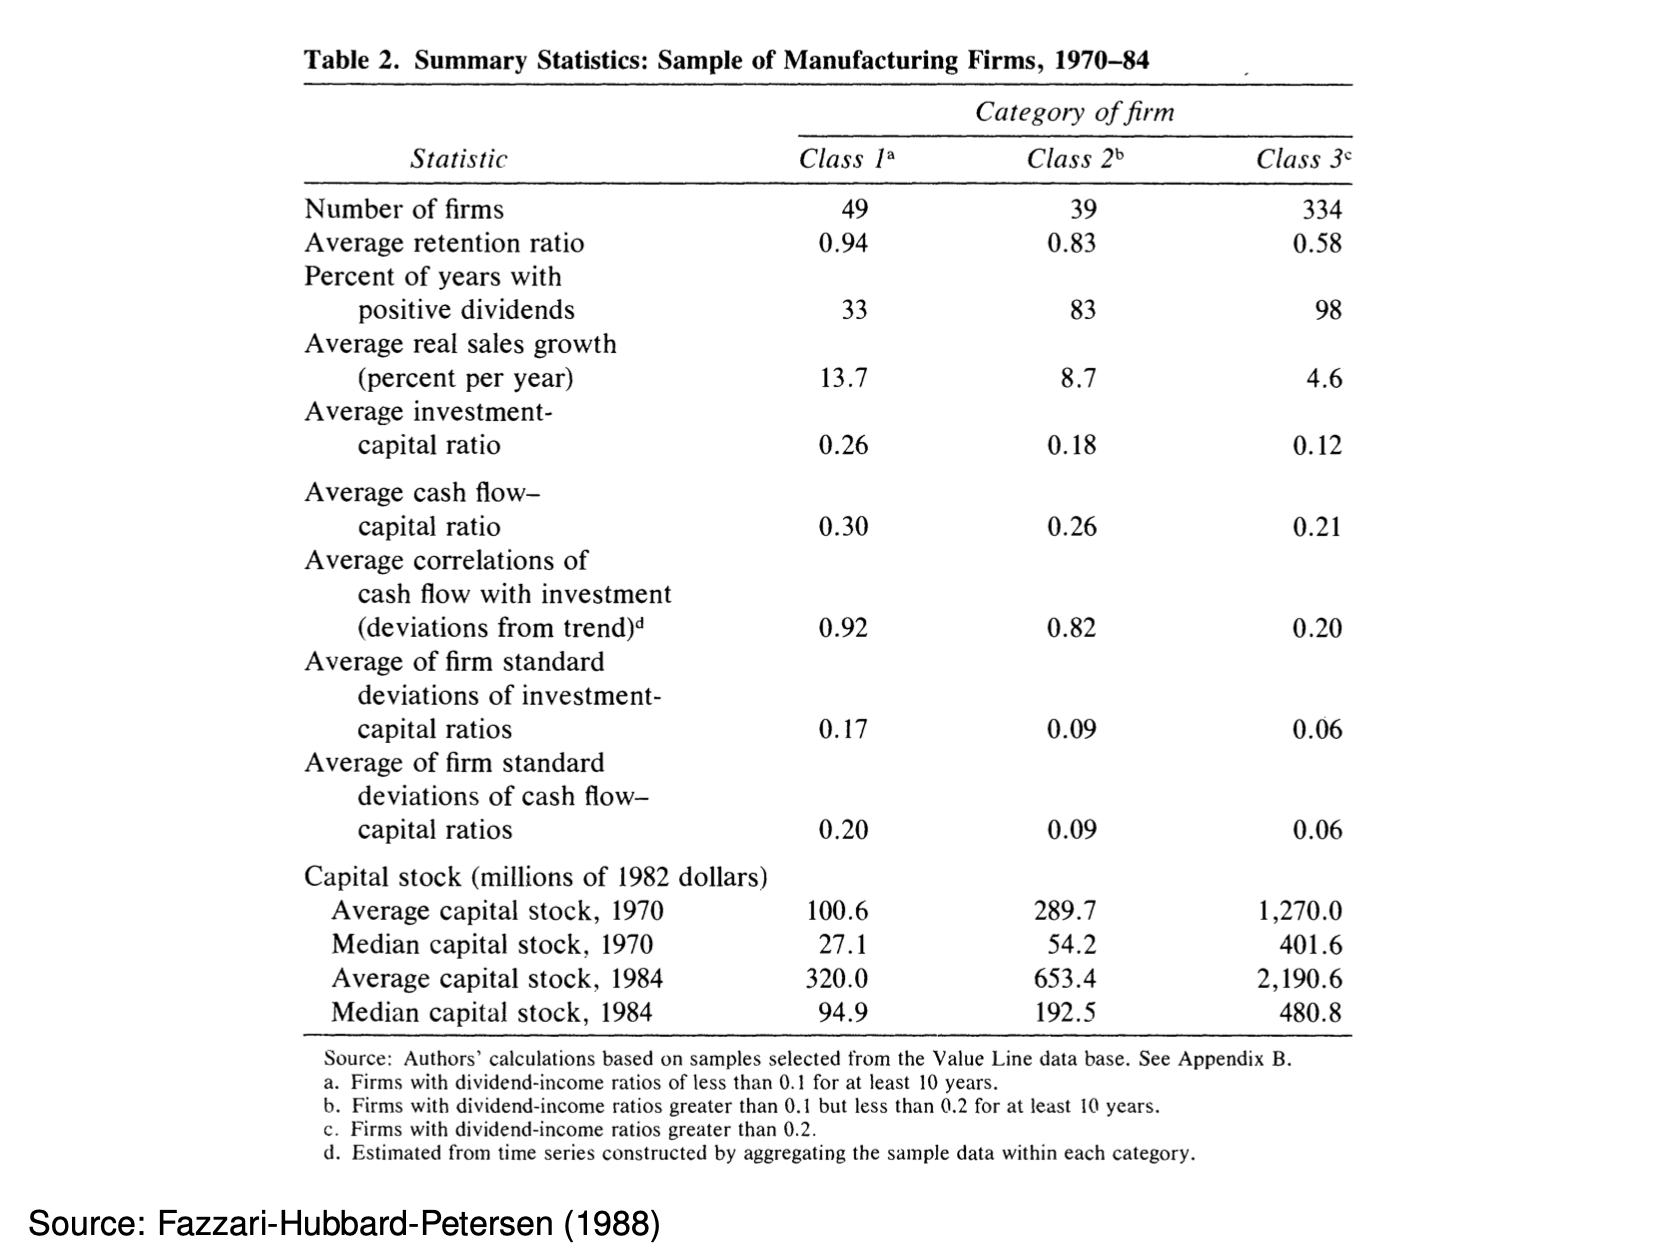
\includegraphics[scale=0.3]{FiguresTables/tab_2_fhp}
\end{figure}
\end{frame}

\begin{frame}{Fazzari Hubbard Petersen (1988)}
\begin{figure}
\centering
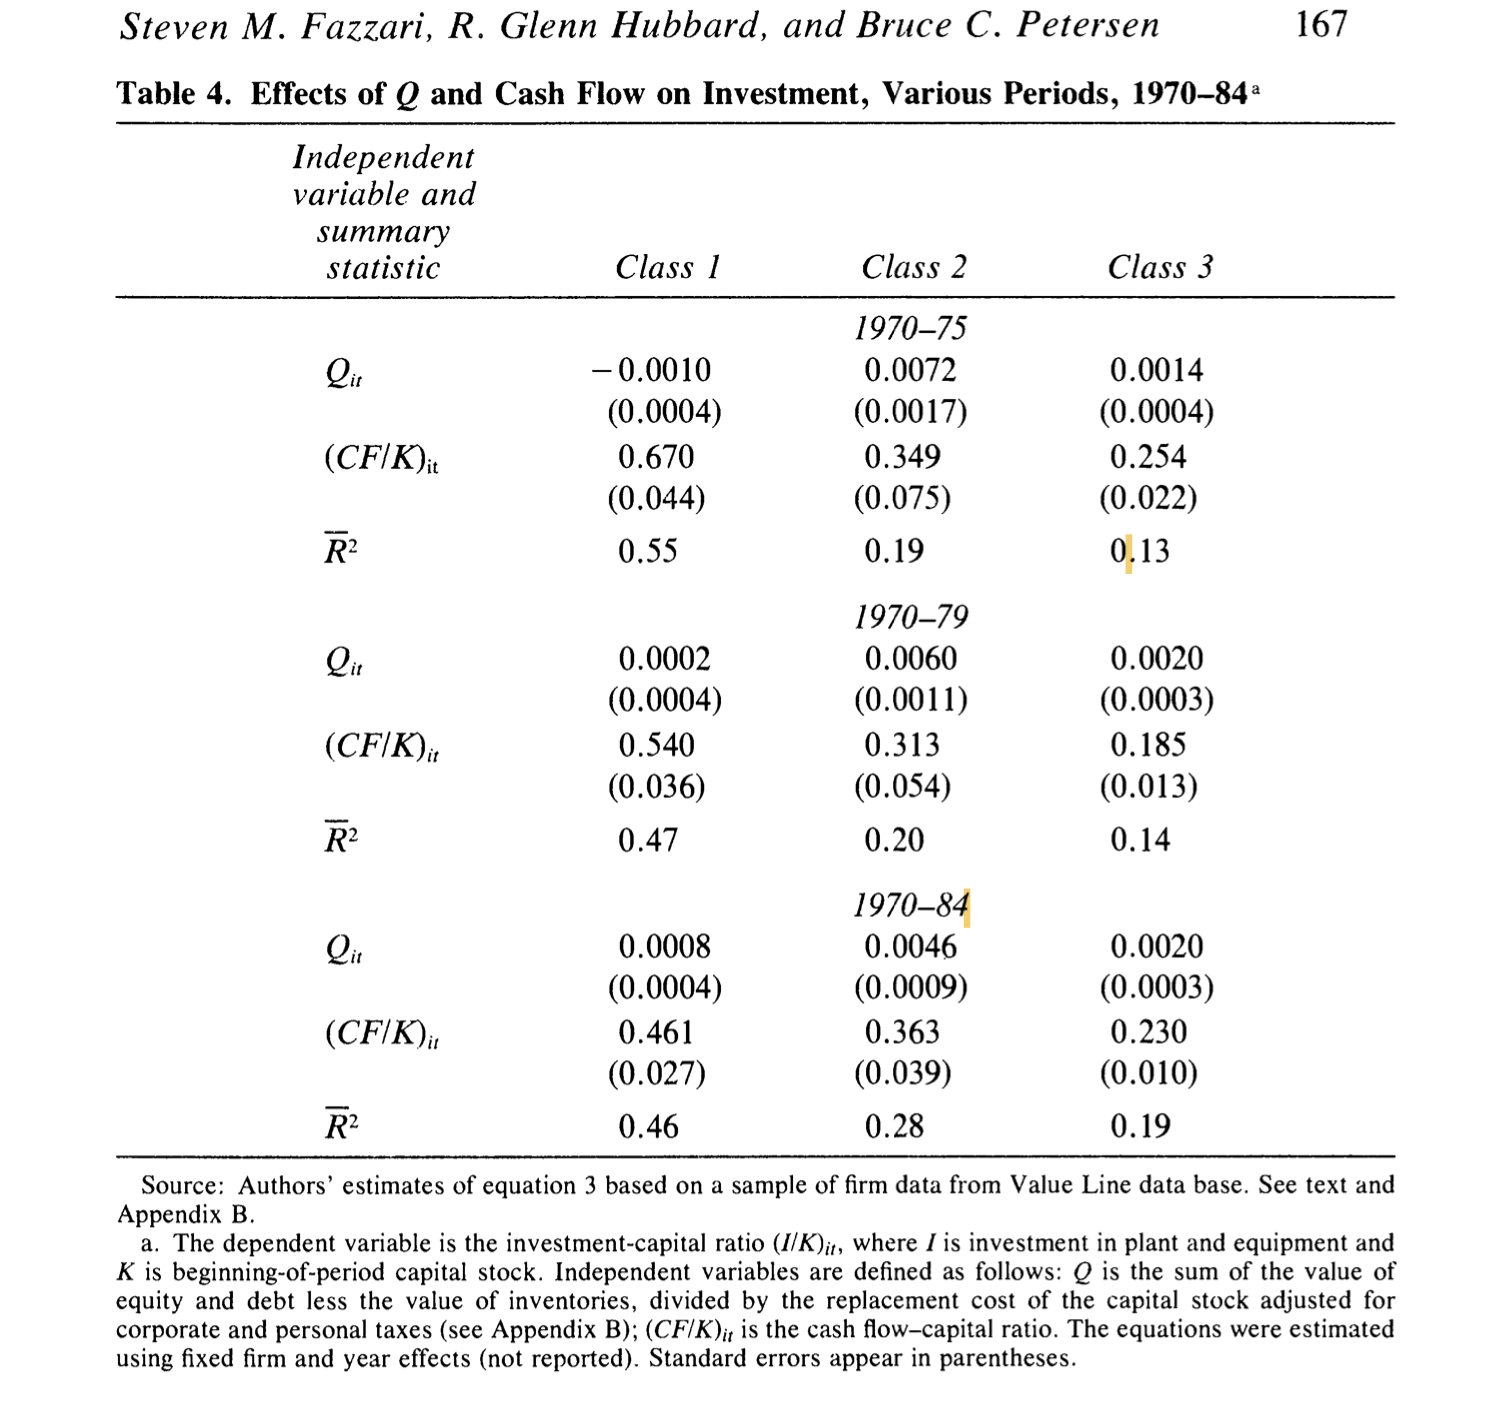
\includegraphics[scale=0.3]{FiguresTables/tab_4_fhp}
\end{figure}
\end{frame}

\begin{frame}{Fazzari Hubbard Petersen (1988)}
\begin{itemize}
\item Recap of main results:
\begin{itemize}
\item Low dividend firms have more sensitivity to cash flows
\item $\beta_1$ very low. Two bad results for the $Q$ theory
\end{itemize}
\item Main threats to identification
\begin{itemize}
\pause
\item $Q$ differentially mismeasured for low dividend firms
\pause
\item Correlation between well-measured $Q$ and $CF$ is higher for low-dividend firms
\end{itemize}
\pause
\item Ideal experiment
\begin{itemize}
\item Find exogenous variation in cash flows
\item Exogenous to future profitability
\end{itemize}
\item Examples
\pause
\begin{itemize}
\item Changes in tax incentives
\item Effects of HQ shocks on subsidiaries
\end{itemize}
\end{itemize}
\end{frame}



\begin{frame}{Temporary Investment Tax Incentives}
\begin{itemize}
	\itemsep1em 
	\item Common form of fiscal stimulus in recessions
	\begin{itemize}
		\item E.g.: 2001-2004, 2008-2011
	\end{itemize}
	\pause
	\item Questions of interest:
	\begin{itemize}
		\item How effective are these policies as stimulus?
		\item What is the response of investment to changes in the cost of capital?
	\end{itemize}
	\item Large literature: {\small Cummins-Hassett-Hubbard (1994), House-Shapiro (2008), Zwick-Mahon (2017)}
\end{itemize}
\end{frame}


\begin{frame}{Bonus Depreciation}
\begin{itemize}
	\itemsep1em 
	\item Firms pay taxes on income net of business expenses
	\pause
	\item Can fully expense wages, advertising, etc. immediately
	\pause
	\item Investment gets expensed over time according to \\ tax depreciation schedules 
	\pause
	\item Bonus depreciation accelerates this depreciation schedule
\end{itemize}
\end{frame}


\begin{frame}
\begin{figure}
	\centering
	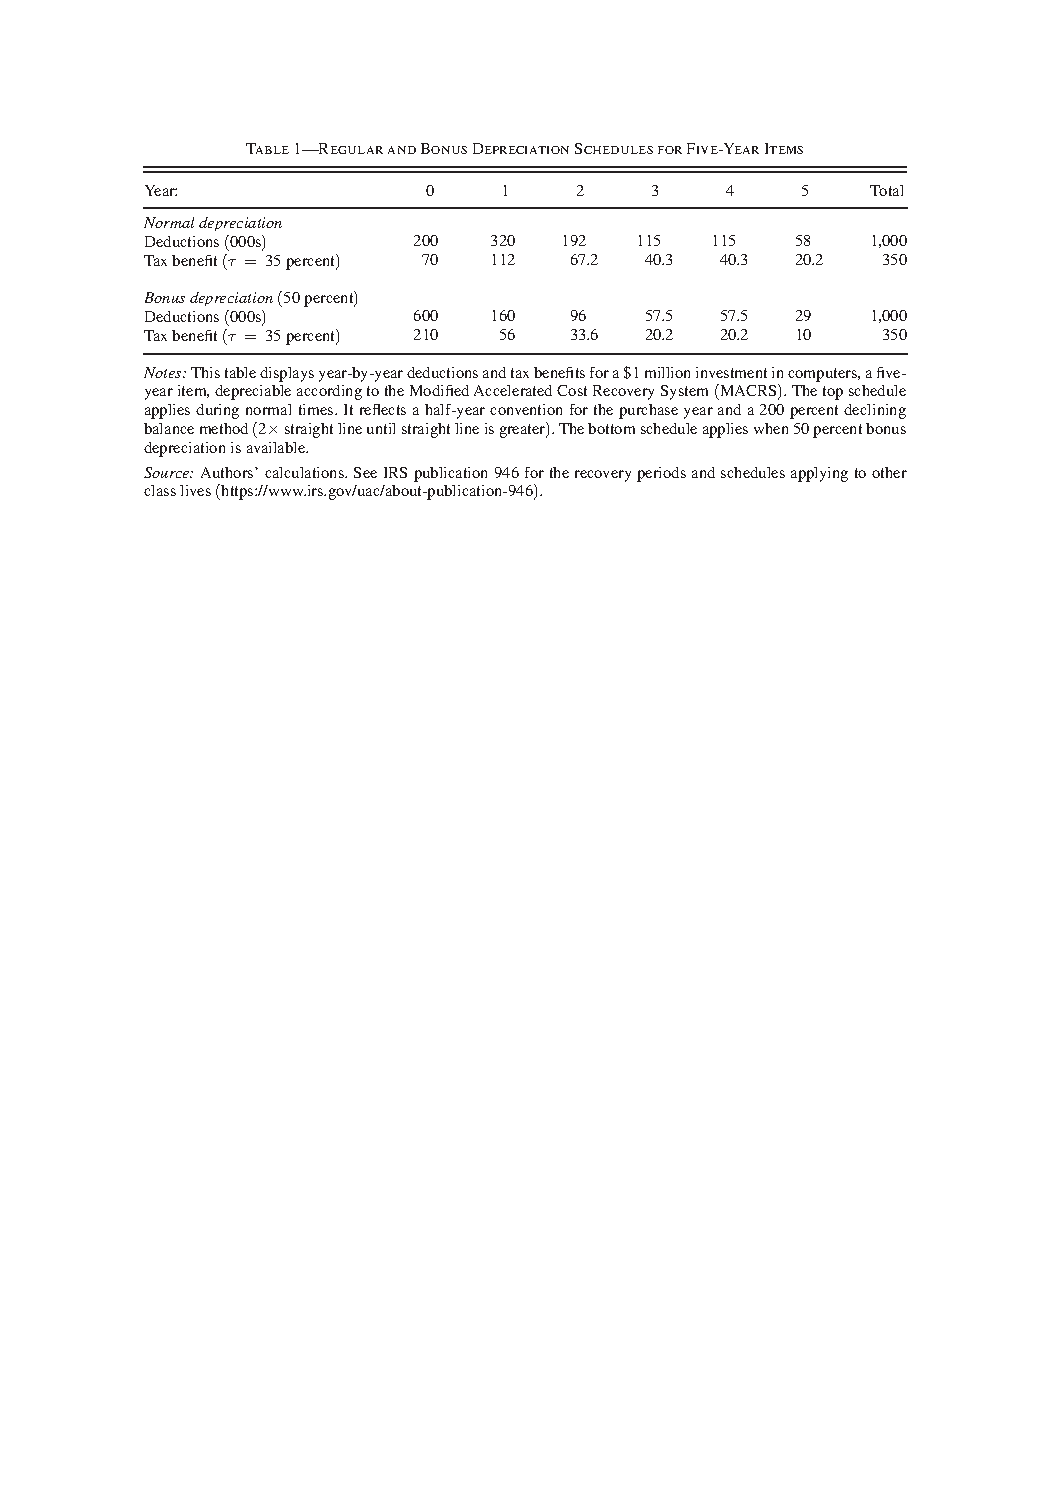
\includegraphics[width=1.0 \textwidth]{FiguresTables/ZwickMahon2017Table1.pdf}
\end{figure}
\vspace{-4mm}
{\scriptsize Source: Zwick-Mahon (2017)}
{\small 
\begin{itemize}
	\item Bonus depreciation allows firm to deduct a per dollar bonus of $\theta$ at the time of investment and the remaining $1-\theta$ according to regular schedule
	\item Table shows bonus depreciation of $\theta = 0.5$
\end{itemize} }
\end{frame}


\begin{frame}{Value of Bonus Depreciation}
Frictionless markets view:
\begin{itemize}
	\item Bonus depreciation only matters due to discounting
	\[ z^0 = D_0 + \sum_{t=1}^{T} \frac{1}{(1+r)^t} D_t \]
	\pause
	\item $D_t$ allowable deduction in period $t$ per dollar of investment in period $0$
	\pause
	\item $r$ risk-adjusted discount rate used by firm
	\pause
	\item Without discounting $z_0 = 1$ (100\%), with discounting $z_0 < 1$
	\pause
	\item Bonus raises $z_0$ by bringing deductions forward in time
	\pause
	\[z = \theta + (1-\theta) z_0 \] 	
\end{itemize}
\end{frame}


\begin{frame}{Value of Bonus Depreciation}
\begin{itemize}
	\itemsep1em 
	\item Frictionless markets view:
	\begin{itemize}
		\item Value of bonus modest for short-lived investments
		\item E.g., with $r = 0.07$, bonus in Table 1 raised $z$ by 2\%
		\item Value of bonus greater for long-lived investments
	\end{itemize}
	\item With financial frictions, bonus may have large effect on investment
	\begin{itemize}
		\item Effect on current cash flow large (\$140,000 in Table 1) 
	\end{itemize}
\end{itemize}
\end{frame}


\begin{frame}{Zwick-Mahon (2017)}
\begin{itemize}
	\itemsep1em 
	\item Estimate the effect of bonus on investment
	\item Bonus occurs in recessions
	\begin{itemize}
		\item Correlated with other determinants of investment
	\end{itemize}
	\item Use difference-in-difference identification strategy
	\begin{itemize}
		\item Bonus more valuable for industries with longer lived investments
		\item Compare effect of bonus on industries with differing duration of investments 
	\end{itemize}
\end{itemize}
\end{frame}


\begin{frame}{Zwick-Mahon (2017): Policy Variable}
\begin{itemize}
	\itemsep1em 
	\item Main policy variable: $z_{N,t}$
	\begin{itemize}
		\item Where $N$ is a 4-digit NAICS industry
	\end{itemize}
	\item Compute baseline $z_N$ for pre-period (1993-2000)
	\begin{itemize}
		\item For each firm-year: weighted average of $z$ across duration categories using a 7\% discount rate
		\item $z_N$ computed as simple average of these firm-year $z$
	\end{itemize}
	\item In bonus years adjust $z_N$ for bonus
	\[z_{N,t} = \theta_t + (1-\theta_t)z_N \]  
\end{itemize}
\end{frame}


\begin{frame}{Zwick-Mahon (2017): Specification}
\begin{itemize}
	\item Baseline difference-in-difference specification:
	\[\log(I_{it}) = \alpha_i + \beta z_{N,t} + \gamma X_{it} + \delta_t + \epsilon_{it} \] \vspace{-15pt} 
	\begin{itemize}
		\item $\beta$ is coefficient of interest
		\item Industry fixed effects: Allow for average differences in industry investment
		\item Time fixed effects: Take out aggregate effects
		\item Industry and time fixed effects are what make this a diff-in-diff 
	\end{itemize}
\end{itemize}
\end{frame}


\begin{frame}{Zwick-Mahon (2017): Identification}
\begin{itemize}
	\itemsep1em 
	\item Identifying assumption: \textbf{Parallel trends}
	\begin{itemize}
		\item Industries with long- and short-duration investment patterns would have evolved in parallel absent bonus
	\end{itemize}
	\item Threat to identification:
	\begin{itemize}
		\item Durable investment industries more resilient in downturns
	\end{itemize}
\end{itemize}
\end{frame}


\begin{frame}
\begin{figure}
	\centering
	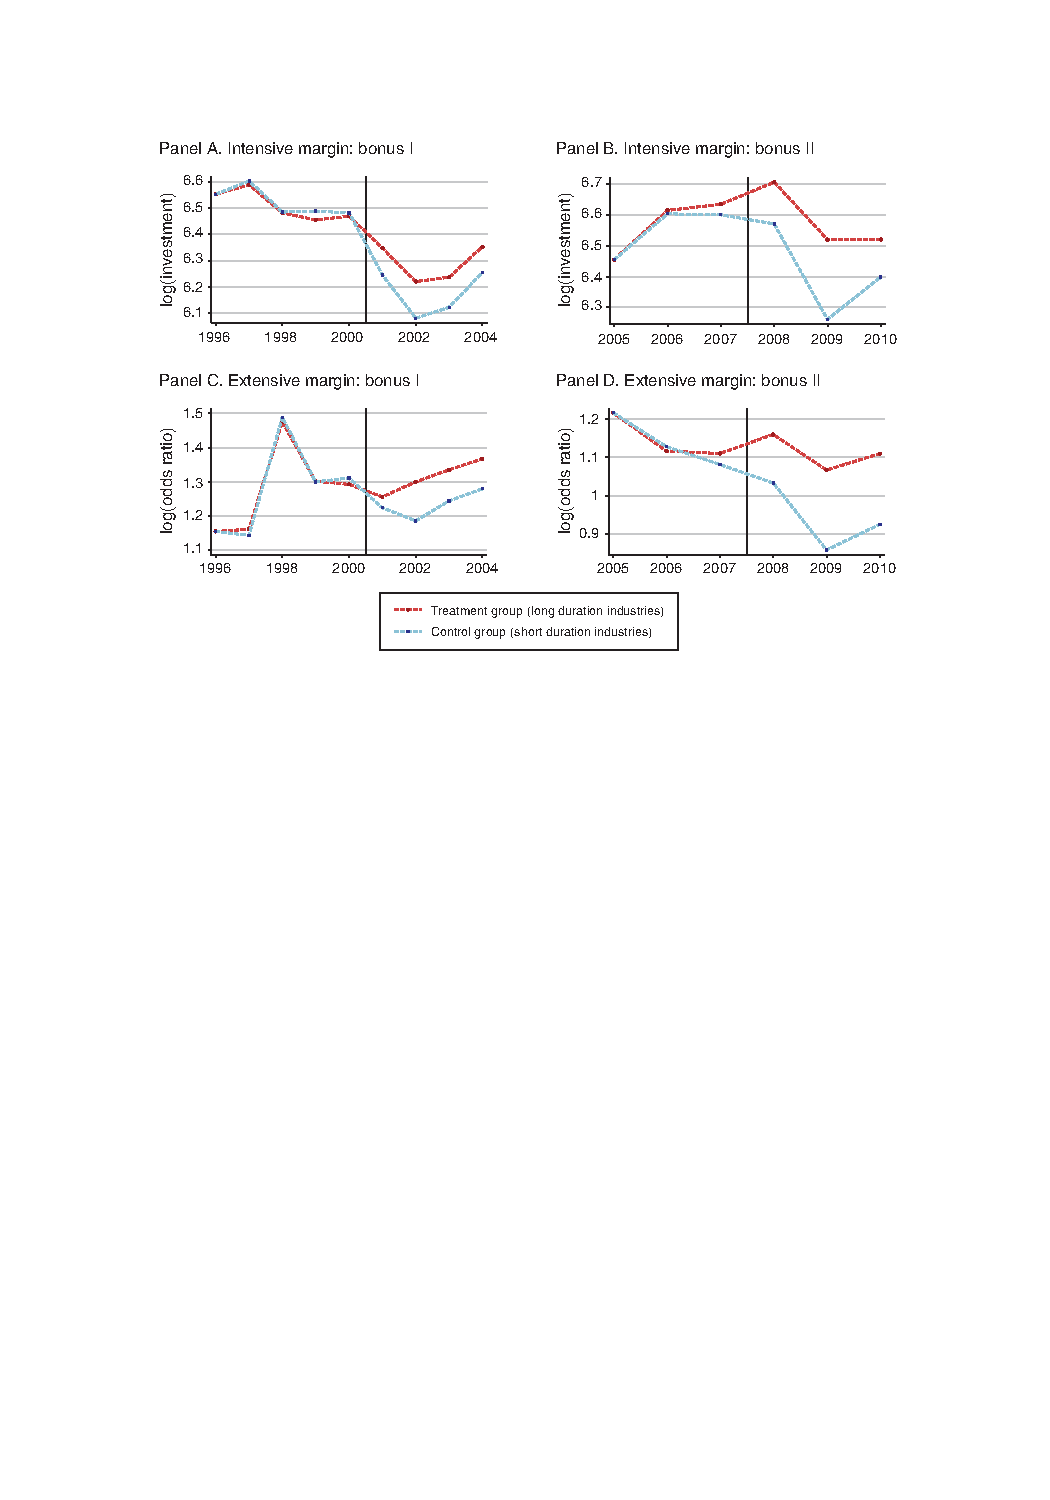
\includegraphics[height=0.85 \textheight]{FiguresTables/ZwickMahon2017Figure1.pdf}
\end{figure}
\vspace{-4mm}
{\scriptsize Source: Zwick-Mahon (2017)}
\end{frame}


\begin{frame}
\begin{figure}
	\centering
	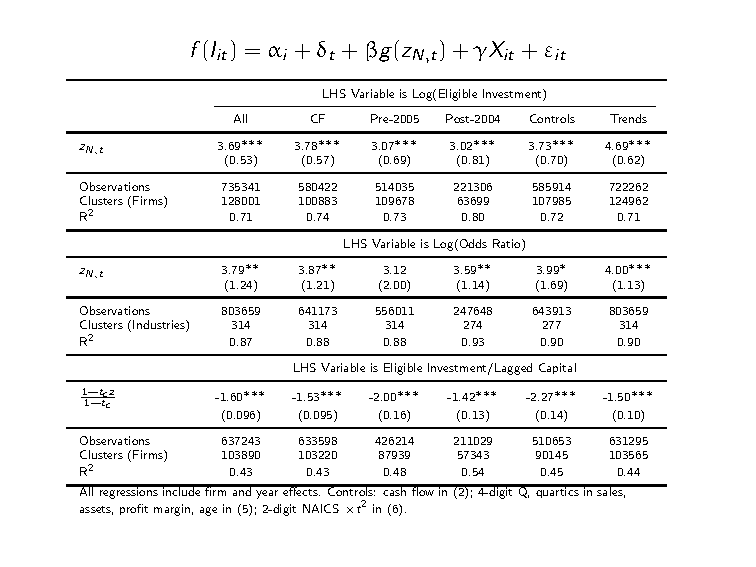
\includegraphics[height=0.9 \textheight]{FiguresTables/ZwickMahon2017Table3.pdf}
\end{figure}
\vspace{-4mm}
{\scriptsize Source: Zwick-Mahon (2017)}
\end{frame}


\begin{frame}{Zwick-Mahon (2017): Effects Are Large}
\begin{itemize}
	\itemsep1em 
	\item Average change in $z_{N,t}$: 
	\begin{itemize}
		\item Early episode: 4.8 cents
		\item Later episode: 7.8 cents
	\end{itemize}
	\item Average change in investment:
	\begin{itemize}
		\item Early episode: 17.7 log points (3.69 x 0.048 = 0.177)
		\item Later episode: 28.8 log points (3.69 x 0.078 = 0.288)	
	\end{itemize}
\end{itemize}
\end{frame}


\begin{frame}{Zwick-Mahon (2017): Effects Are Large}
\begin{itemize}
	\itemsep1em 
	\item In simple investment model:
	\begin{itemize}
		\item Elasticity of investment with respect to net of tax rate, $1-\tau z$, \\ equals price and interest elasticity
	\end{itemize}
	\[ \log (I_{it}) = \alpha + \beta \log(1-\tau z_{N,t}) + \epsilon_{it} \]
	\item Zwick-Mahon's regressor is $z_{N,t}$ not $\log(1-\tau z_{N,t})$
	\item Linear approximation:
	\[ \log(1-\tau z_{N,t}) =  \log(1-\tau z_{N}) - \frac{\tau}{1-\tau z_{N}} (z_{N,t} - z_N)  \] 
	\item Zwick-Mahon results imply price and interest rate elasticities \\ of investment equal to
	\[- 3.69 \div \frac{\tau}{1-\tau z} \approx -7.2 \] 
\end{itemize}
\end{frame}


\begin{frame}
\begin{figure}
	\centering
	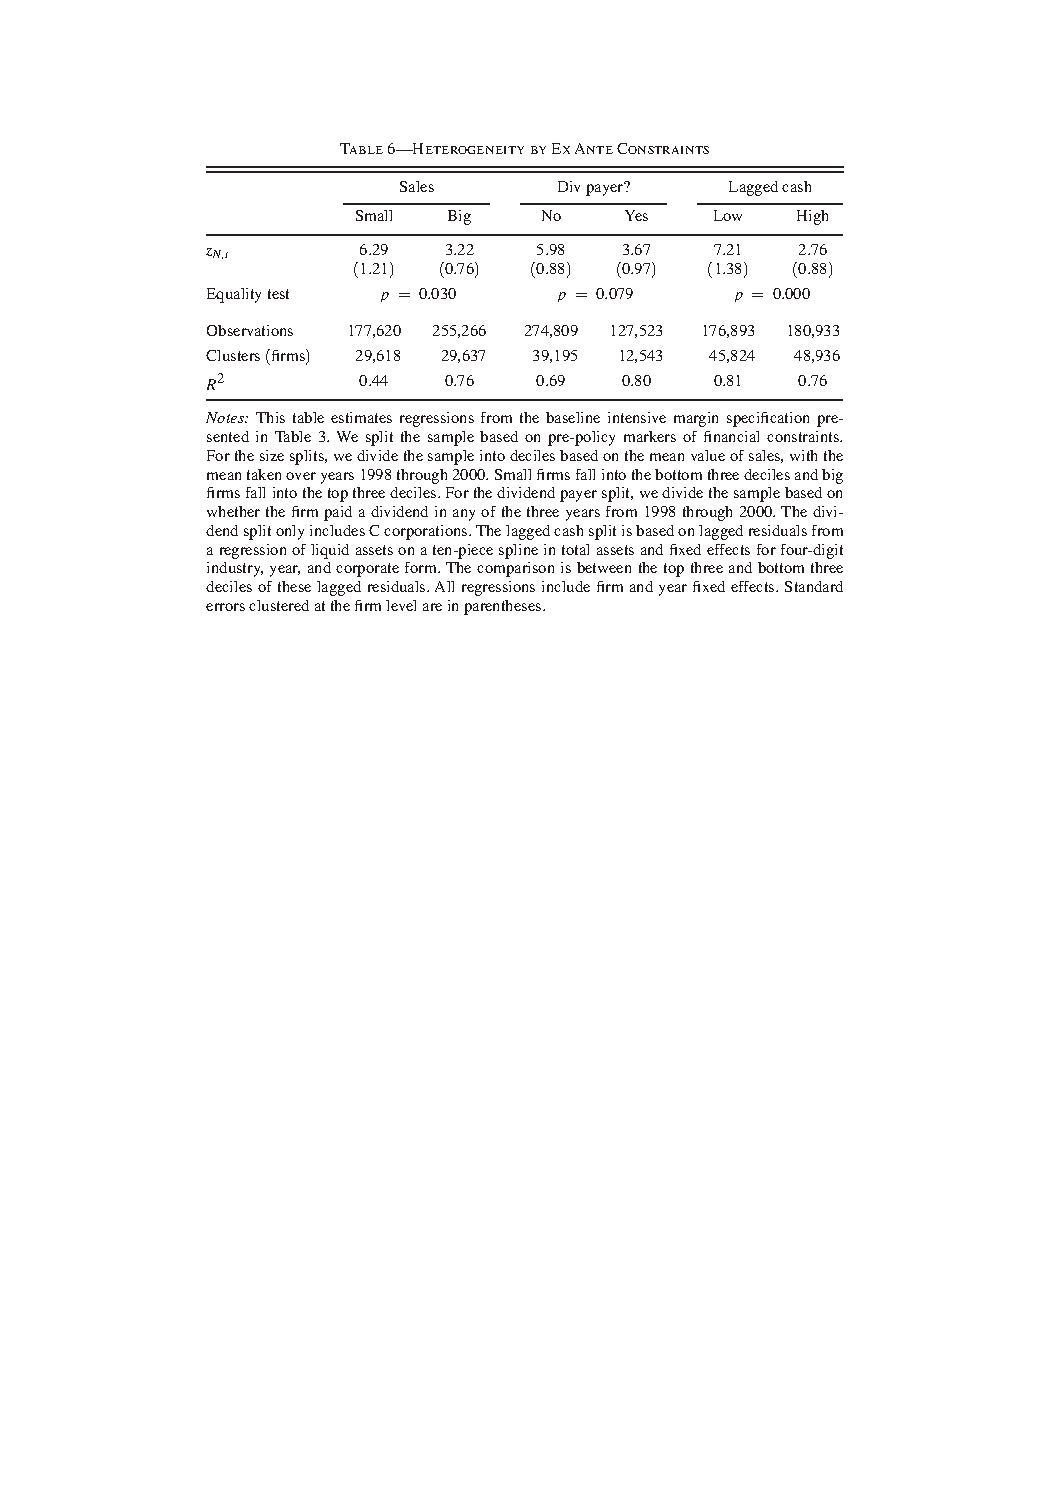
\includegraphics[height=0.85 \textheight]{FiguresTables/ZwickMahon2017Table6.pdf}
\end{figure}
\vspace{-4mm}
{\scriptsize Source: Zwick-Mahon (2017)}
\end{frame}


\begin{frame}
\begin{figure}
	\centering
	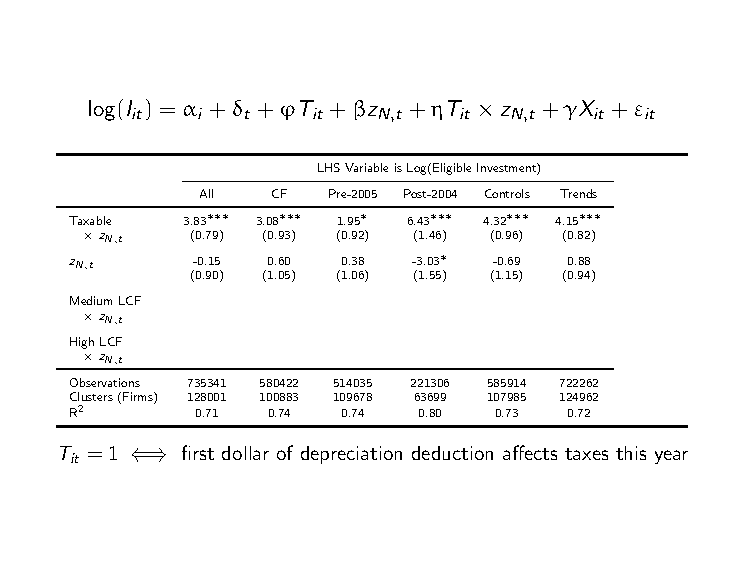
\includegraphics[height=0.8 \textheight]{FiguresTables/ZwickMahon2017Table7.pdf}
\end{figure}
\vspace{-6mm}
{\scriptsize Source: Zwick-Mahon (2017)}
\end{frame}


\begin{frame}{Heterogeneity in Effect}
\begin{itemize}
	\itemsep1em 
	\item More liquidity constrained firms have larger effects
	\item Effect only exists for firms with immediate tax benefit
	\item[]
	\item Concern: Firms with neg. earning may have worse growth prospects
	\begin{itemize}
		\item Redo analysis including only firms close to zero earning
	\end{itemize}
\end{itemize}
\end{frame}


\begin{frame}{Micro-Foundation for Adjustment Costs}
\begin{itemize}
	\itemsep1em 
	\item Adjustment cost function is a black box
	\item Crucial aspect of the theory, but we don't know what it is
	\item Some possibilities that explain the ZM results
	\begin{itemize}
		\item Financial frictions
		\item Fixed costs of adjustment
	\end{itemize}
\end{itemize}
\end{frame}


\end{document}








